\documentclass[letterpaper,twocolumn,10pt]{article}

% OSDI/USENIX submission geometry: US Letter, two columns, 7" x 9" text block,
% 0.33" column gutter, 10pt body on approximately 12pt leading.
\usepackage[letterpaper,textwidth=7in,textheight=9in,centering]{geometry}
\setlength{\columnsep}{0.33in}
\linespread{1.03}

\usepackage{fontspec}
\usepackage{xeCJK}
\setmainfont{TeX Gyre Termes}
\setsansfont{TeX Gyre Heros}
\setmonofont{DejaVu Sans Mono}[Scale=0.86]
\setCJKmainfont{Noto Serif CJK SC}
\setCJKsansfont{Noto Sans CJK SC}
\setCJKmonofont{Noto Sans Mono CJK SC}

\usepackage{microtype}
\usepackage{graphicx}
\usepackage{booktabs}
\usepackage{multirow}
\usepackage{tabularx}
\usepackage{amsmath}
\usepackage{amssymb}
\usepackage{enumitem}
\usepackage{xspace}
\usepackage{xcolor}
\usepackage{listings}
\usepackage{tikz}
\usepackage{caption}
\usepackage{subcaption}
\usepackage{placeins}
\usepackage{url}
\usepackage[hidelinks]{hyperref}
\usetikzlibrary{arrows.meta,positioning,shapes.geometric,fit,calc}

\pagestyle{plain}
\setlength{\parskip}{0pt}
\setlength{\parindent}{1em}
\setlist{leftmargin=*,nosep}
\captionsetup{font=small,labelfont=bf}
\newcommand{\sys}{\textsc{BPFix}\xspace}
\newcommand{\code}[1]{\texttt{#1}}
\newcolumntype{Y}{>{\raggedright\arraybackslash}X}

\lstdefinestyle{tinycode}{
  basicstyle=\ttfamily\scriptsize,
  breaklines=true,
  columns=fullflexible,
  keepspaces=true,
  frame=single,
  framerule=0.2pt,
  xleftmargin=2pt,
  xrightmargin=2pt,
  aboveskip=4pt,
  belowskip=4pt,
}

\lstdefinestyle{ccode}{
  language=C,
  basicstyle=\ttfamily\scriptsize,
  keywordstyle=\bfseries,
  commentstyle=\itshape\color{gray!70!black},
  breaklines=true,
  columns=fullflexible,
  keepspaces=true,
  frame=single,
  framerule=0.2pt,
  numbers=left,
  numberstyle=\tiny\color{gray!70!black},
  numbersep=4pt,
  aboveskip=4pt,
  belowskip=4pt,
}

\title{\Large\bf
\sys：面向 eBPF Verifier 失败的证明生命周期诊断系统}

\author{
  {\rm Anonymous Authors}\\
  Paper draft for OSDI-style review
}

\date{}

\begin{document}
\maketitle

\begin{abstract}
eBPF 已经成为 Linux 内核中网络、安全、可观测性和存储扩展的事实标准，但每个 eBPF 程序在执行前都必须通过内核 verifier。Verifier 的安全检查基于抽象解释，能够阻止越界访问、未初始化栈读取、引用泄漏和不受控循环；同时，它的失败日志往往是几百到几千行寄存器抽象状态，开发者通常只能看到最后一条拒绝消息，而不知道安全证明在哪里建立、在哪里丢失、为什么最终无法被 verifier 接受。

本文提出 \sys，一个完全运行在用户态的 verifier 失败诊断系统。我们的核心观察是：verbose verifier log 不是普通调试文本，而是一条 verifier 证明尝试的轨迹。通过解析每条 BPF 指令处的寄存器类型、标量边界、指针范围、引用状态和源码注释，\sys 将最终错误还原为一个 required proof，并沿轨迹重建证明生命周期：证明从未建立、证明已经建立但在 lowering 后丢失、证明在控制流合并处变弱，或证明受限于内核环境和 verifier 预算。基于这一表示，\sys 输出类似 Rust 编译器的 multi-span 诊断和稳定 JSON，使本地调试、CI 标注、编辑器和自动化 agent 能够直接消费。

我们实现了一个 Rust CLI 和可复现实验语料库。当前 \code{bpfix-bench} 包含 235 个可本地 replay 的 verifier-reject 案例，覆盖 Stack Overflow、GitHub issue、GitHub commit 和 Linux kernel selftest。本文给出对这些失败的 characterization，说明真实用户遇到的 verifier 问题不是单一的“缺少 bounds check”，而是源代码缺陷、编译器 lowering artifact、环境配置、verifier false positive 和 verifier 资源限制的混合。在 60-case blind audit 中，两个独立 scorer 都认为 \sys 是唯一能稳定给出 root localization 和 correct help 的方法，但也指出 14/60 case 仍有 unsafe help。我们的设计目标不是替换 verifier，也不是自动改代码，而是在保持现有 eBPF 工作流不变的前提下，把 opaque verifier log 转换成开发者下一步能行动的证明解释。
\end{abstract}

\section{引言}

eBPF 允许开发者在不修改内核源码、不重启系统的情况下把小型程序加载到内核关键路径中。生产系统用它实现网络策略、负载均衡、安全审计、性能追踪和运行时可观测性。这个能力的前提是内核 verifier：每个程序在运行前必须被静态检查，证明它不会越界访问内核或包数据、不会读取未初始化栈、不会泄漏 verifier 跟踪的引用、不会在不可终止路径上消耗任意资源。

Verifier 的能力强，代价也高。失败时，开发者看到的是一段面向 verifier 维护者的抽象状态日志，而不是面向程序作者的诊断。真实日志通常包含数百行如下信息：寄存器 \code{R1..R10} 的类型、\code{umin/umax}、\code{smin/smax}、\code{var\_off}、packet range、map value range、frame pointer offset、引用 id、\code{mark\_precise} 回溯和 BTF 源码注释。最后一行可能只是“\code{R5 invalid mem access 'scalar'}”或“\code{math between pkt pointer and register with unbounded min value is not allowed}”。这些消息说明 verifier 在哪里停止，却不说明开发者需要怎样的安全证明、这个证明是否曾经存在、它在哪里被编译器或控制流转换破坏。

现有工具没有把这个问题当作“证明诊断”来处理。Pretty Verifier 一类工具主要把最终错误文本重写成人类可读提示；LLM agent 可以读整段日志，但缺少稳定的结构化事实和可验证输出；Rex 等系统指出了语言和 verifier 之间的 gap，但目标是提供新的可用内核扩展语言，而不是诊断现有 C/Rust/Aya/libbpf 工作流中的 verifier reject~\cite{rex2025,kgent2024,prettyverifier2025}。本文的立场更小、更工程化：保留现有 eBPF 工具链，直接读取开发者已经拥有的 verifier log，输出下一步能改代码、改环境或定位 verifier 限制的诊断。

\sys 的关键洞察是，verbose verifier log 是一条证明尝试轨迹。Verifier 在每条指令处都记录抽象状态；一个失败不是单点事件，而是 required proof 的生命周期事件。对于 packet access，required proof 是“访问处寄存器仍是 packet pointer，且 \code{off + size <= range}”；对于 nullable map value，required proof 是“使用处已经在同一个 verifier 可见分支内排除了 null”；对于引用泄漏，required proof 是“每条退出路径释放对应 reference id”。\sys 将最终错误和拒绝点状态实例化为 required proof，然后沿轨迹寻找证明建立、保持、丢失和拒绝的位置。

这一表示带来两个用户可见收益。第一，它让诊断从“最后错误字符串”升级为 multi-span 解释：哪一行源码建立了 bounds/null/reference proof，哪条 BPF 指令或源码 lowering 让 verifier 丢失该事实，最终哪一行因此被拒绝。第二，它把失败分类和 triage 变成可解释结果：如果 proof 从未建立，通常是 source bug；如果 proof 建立后被 shift/or/cast/branch merge 等 lowering 破坏，通常是 lowering artifact；如果缺少 helper、BTF、kernel feature，则是 environment/configuration；如果 verifier 预算耗尽，则是 verifier limit。

表~\ref{tab:positioning} 将 \sys 放在现有诊断路径中。它的目标不是替代语言、loader 或 verifier，而是在现有日志和用户之间补一个 proof-aware diagnosis 层。

\begin{table*}[t]
\centering
\small
\caption{\sys 与现有诊断路径的区别。核心差异是是否把 verifier log 当作可分析的 proof trace。}
\label{tab:positioning}
\begin{tabularx}{\textwidth}{@{}l X X X@{}}
\toprule
方法 & 输入 & 输出 & 主要限制 \\
\midrule
Raw verifier log & kernel/libbpf 原始 verbose log & 最终错误和寄存器状态文本 & 信息完整但不解释 proof lifecycle；用户要手动读抽象状态 \\
Message translator & 最终错误或少量上下文 & 人类可读错误说明 & 通常只重写 symptom，不知道 proof 是否曾建立或丢失 \\
LLM + raw log & 整段日志和可选源码 & 自然语言解释 & 输出不稳定，难保证 schema、grounding 和 no-oracle 评估 \\
Rex 等语言系统 & 新语言或受控 runtime & 避免部分 language-verifier gap & 需要改变开发模型；不服务现有失败日志 \\
\sys & verifier/build log + optional object & multi-span proof diagnostic + JSON & 依赖日志质量；当前 error catalog 和 proof-span 覆盖仍在扩展 \\
\bottomrule
\end{tabularx}
\end{table*}

\begin{figure*}[t]
\centering
\begin{subfigure}[t]{0.31\textwidth}
\textbf{A. 用户源码}
\begin{lstlisting}[style=ccode]
void *data = (void *)(long)ctx->data;
void *end  = (void *)(long)ctx->data_end;

if (data + sizeof(struct hdr) > end)
    return XDP_DROP;

struct hdr *h = data;
__u16 len = bpf_ntohs(h->len);
data += len;          // verifier rejects
\end{lstlisting}
\end{subfigure}
\hfill
\begin{subfigure}[t]{0.32\textwidth}
\textbf{B. 原始 verifier 摘要}
\begin{lstlisting}[style=tinycode]
22: R0_w=inv(umax=65280,var_off=...)
    R6_w=inv(umax=255,var_off=...)
22: (4f) r0 |= r6
23: R0_w=inv(id=0)
...
math between pkt pointer and register
with unbounded min value is not allowed
\end{lstlisting}
\end{subfigure}
\hfill
\begin{subfigure}[t]{0.32\textwidth}
\textbf{C. \sys 输出}
\begin{lstlisting}[style=tinycode]
error[BPFIX-E005]: scalar range proof is missing
  --> xdp.c:8
4 | if (data + sizeof(struct hdr) > end)
  | proof established: packet range checked
7 | __u16 len = bpf_ntohs(h->len);
  | proof lost: OR collapses scalar bound
8 | data += len;
  | rejected: pkt pointer + unbounded scalar
  = required proof: prove non-negative bounded scalar
help: mask or clamp len before pointer arithmetic
\end{lstlisting}
\end{subfigure}
\caption{Verifier 失败的用户体验差异。原始日志说明 verifier 停在哪里；\sys 把日志解释成证明生命周期：证明建立、证明丢失、最终拒绝。}
\label{fig:motivation}
\end{figure*}

本文贡献如下：
\begin{itemize}
  \item 我们对一个可 replay 的 eBPF verifier reject 语料库做 characterization，展示真实失败由源代码证明缺失、lowering artifact、环境配置、verifier false positive 和 verifier limit 混合构成。
  \item 我们提出 proof lifecycle diagnostic：从最终拒绝重建 required proof，并在 verifier 抽象状态轨迹中定位 proof established、proof lost、rejected 等事件。
  \item 我们实现 \sys，一个用户态 Rust CLI，默认输入 verifier/build/bpftool/libbpf/Aya/BCC 日志、默认输出 plain text 诊断，并提供 JSON 用于 CI、编辑器和 agent。
  \item 我们给出面向开源工具的 artifact 设计：\code{bpfix [LOG]} 主路径、可复现 benchmark、跨工具 examples，以及稳定诊断 schema。
\end{itemize}

\section{背景与问题}

\subsection{Verifier 的抽象状态}

Linux eBPF verifier 是一个路径敏感的抽象解释器~\cite{gershuni2019simple,cousot1977}。它不执行程序，而是在 BPF 字节码层维护抽象状态。每个寄存器可能是 scalar、packet pointer、map value pointer、frame pointer、context pointer、dynptr、reference 等；scalar 有 signed/unsigned range 和 \code{tnum}；pointer 有固定 offset、变量 offset、可访问 range 和 provenance id。Verifier 接受程序的条件不是“源代码看起来安全”，而是“在每个被检查的字节码指令处，当前抽象状态足以证明所需安全条件”。

这种设计导致源码和 verifier 之间存在语义错位。开发者写的是 C、Rust、Aya 或 BCC 程序；LLVM、libbpf skeleton 或框架宏会改写控制流、表达式和寄存器分配；verifier 最终只看到 BPF 指令和寄存器状态。一个源代码 bounds check 可以在源码层完全合理，却在字节码层因为分支合并、整数转换、helper 参数传递或 bitwise 操作变成 verifier 无法追踪的抽象状态。

\subsection{为什么最终错误不够}

最终错误行是 verifier 的失败断言，不是诊断。它告诉我们“这个 access 处没有 proof”，但不告诉我们：
\begin{enumerate}
  \item proof 是否曾经建立；
  \item 如果建立过，是哪条转换破坏了它；
  \item 破坏来自用户代码、编译器 lowering、内核能力还是 verifier 预算；
  \item 用户下一步应该改源码、换内核配置、缩小程序，还是报告 verifier bug。
\end{enumerate}

图~\ref{fig:motivation} 展示了典型 lowering artifact。最后错误是 scalar unbounded，但根因是 \code{bpf\_ntohs} lowering 后的 OR 操作使 verifier 丢失 scalar bound。只提示“给 scalar 加 bounds check”容易误导用户，因为源码中确实已有 packet bounds check；更有用的提示是指出 proof 在 byte-swap lowering 中被破坏，建议在 pointer arithmetic 前显式 mask/clamp 或重新组织代码。

\subsection{用户体验目标}

\sys 的 UX 目标刻意简单：输入 verifier log，输出 plain text 诊断。用户不应先理解 benchmark、标签体系或 verifier 源码。典型命令应是：
\begin{lstlisting}[style=tinycode]
bpfix verifier.log
make load 2>&1 | bpfix
sudo bpftool -d prog load xdp.o /sys/fs/bpf/xdp 2>&1 | bpfix
\end{lstlisting}
只有当另一个工具要消费结果时，才使用 \code{--format json}；只有当用户手头有 BPF object 且希望增强 bytecode/source correlation 时，才使用 \code{--object prog.o}。这一设计把 \sys 定位为现有 eBPF 工作流旁边的诊断层，而不是新的 loader、语言或 verifier。

\section{失败 Characterization}
\label{sec:characterization}

为了让诊断系统面向真实用户问题，而不是少数手工例子，我们构建了 \code{bpfix-bench}：一个可以在本地 replay 的 verifier reject corpus。每个 case 都包含源程序、构建脚本、load/replay 命令和期望的 verifier reject。Validator 会重新构建对象、加载程序、捕获新的 verifier log，并确认当前内核确实拒绝该程序。这样得到的 case 是“今天这台机器上可重现的失败”，而不是历史 issue 中不可复现的文本片段。

\begin{table}[t]
\centering
\caption{\code{bpfix-bench} 当前 replayable cases 来源组成。}
\label{tab:bench-source}
\begin{tabular}{lrr}
\toprule
来源 & cases & 占比 \\
\midrule
Stack Overflow & 86 & 36.6\% \\
Linux kernel selftest & 85 & 36.2\% \\
GitHub commit & 46 & 19.6\% \\
GitHub issue & 18 & 7.7\% \\
\midrule
总计 & 235 & 100\% \\
\bottomrule
\end{tabular}
\end{table}

\begin{table}[t]
\centering
\small
\caption{Raw external audit 到 primary benchmark 的筛选状态。Raw records 是扩展候选和审计材料；只有 fresh replay 成功的 case 才进入主指标。}
\label{tab:raw-funnel}
\begin{tabularx}{\columnwidth}{@{}l r X@{}}
\toprule
raw 状态 & records & 含义 \\
\midrule
\code{replay\_valid} & 150 & 外部记录可重建 verifier reject \\
\code{environment\_required} & 197 & 依赖特定 kernel/helper/BTF 或运行环境 \\
\code{attempted\_accepted} & 32 & 当前环境接受，不能作为 reject case \\
\code{missing\_source} & 31 & 缺少可构建源码 \\
\code{missing\_verifier\_log} & 15 & 缺少可核对的 verifier log \\
\code{not\_reconstructable} & 45 & diff/issue 信息不足以重建 \\
\code{out\_of\_scope} & 262 & 非 verifier reject 或不适合主指标 \\
\bottomrule
\end{tabularx}
\end{table}

\begin{table}[t]
\centering
\small
\caption{Primary taxonomy 显示 verifier reject 的根因不是单一类型。}
\label{tab:taxonomy}
\begin{tabularx}{\columnwidth}{@{}l r X@{}}
\toprule
根因类别 & cases & 解释 \\
\midrule
source bug & 187 & 源码没有给出 verifier 所需证明 \\
lowering artifact & 24 & 源码意图合理，lowering 后 proof 丢失 \\
environment & 11 & kernel/helper/BTF/配置不匹配 \\
false positive & 9 & verifier 保守或 bug 导致拒绝 \\
verifier limit & 4 & instruction/state/loop/stack 预算限制 \\
\bottomrule
\end{tabularx}
\end{table}

表~\ref{tab:bench-source} 和表~\ref{tab:taxonomy} 给出当前 corpus 快照。235 个 replayable case 覆盖四类来源，其中 kernel selftest 提供了复杂、现代、接近 verifier 维护者关注点的失败，Stack Overflow 和 GitHub issue/commit 则代表普通用户和真实项目遇到的问题。表~\ref{tab:raw-funnel} 显示 raw audit 并没有直接进入主指标：大量外部记录因为环境绑定、缺源码、缺 verifier log 或不属于 verifier reject 被排除。Taxonomy 上，source bug 占多数，但 lowering artifact、环境配置、false positive 和 verifier limit 合计达到 48 个 case；图~\ref{fig:taxonomy-bars} 把这个长尾更直观地展示出来。这说明一个只会输出“加 bounds check”的工具不够；真实诊断必须区分“缺 proof”和“proof 丢了”。

\begin{figure}[t]
\centering
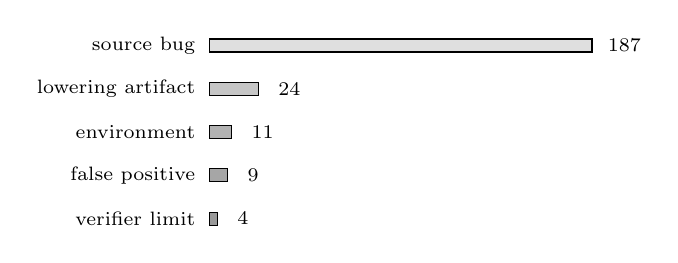
\begin{tikzpicture}[
  bar/.style={draw=black, fill=gray!25, minimum height=0.28cm},
  label/.style={font=\scriptsize, anchor=east},
  val/.style={font=\scriptsize, anchor=west},
  x=0.026cm,y=0.55cm
]
\node[label] at (0,0) {source bug};
\draw[bar] (2, -0.15) rectangle +(187,0.3);
\node[val] at (192,0) {187};
\node[label] at (0,-1) {lowering artifact};
\draw[bar,fill=gray!45] (2, -1.15) rectangle +(24,0.3);
\node[val] at (31,-1) {24};
\node[label] at (0,-2) {environment};
\draw[bar,fill=gray!60] (2, -2.15) rectangle +(11,0.3);
\node[val] at (18,-2) {11};
\node[label] at (0,-3) {false positive};
\draw[bar,fill=gray!70] (2, -3.15) rectangle +(9,0.3);
\node[val] at (16,-3) {9};
\node[label] at (0,-4) {verifier limit};
\draw[bar,fill=gray!80] (2, -4.15) rectangle +(4,0.3);
\node[val] at (11,-4) {4};
\end{tikzpicture}
\caption{Replayable corpus 的根因分布。非源码缺陷类失败足够常见，必须在诊断中明确区分。}
\label{fig:taxonomy-bars}
\end{figure}

\subsection{Characterization 发现}

\textbf{标注流程。}
每个 admitted case 的 \code{case.yaml} 包含 \code{taxonomy\_class}、mechanism tags、evidence tags、root-cause description、fix direction 和 confidence。标签来源分为四类：外部记录重建（105 个）、自动/人工一致的 agree 标签（104 个）、manual reconstruction（17 个）和 adjudicated（9 个）。Confidence 分布为 high 94、medium 137、low 4；当前 taxonomy headline 包含全部 replayable cases，但 evaluation 中需要对 low-confidence case 单独报告敏感性分析。我们不把 raw issue 文本直接作为 ground truth；只有 replay capture、terminal verifier error 和 case-level evidence 一致时，case 才进入 primary corpus。
表~\ref{tab:label-provenance} 给出这些标签的来源，用来区分 replay-derived evidence 和人工裁决边界样本。表~\ref{tab:taxonomy-rubric} 给出标注规则：同一个 terminal error 可以落入不同 taxonomy，裁决依据是 replay evidence、源码 proof 是否存在、修复是否改变语义前置条件，以及是否需要换环境或缩小 verifier 状态空间。

\begin{table}[t]
\centering
\small
\caption{Case label provenance。多数标签来自 replay reconstruction 或 agree path，少量 case 经过 adjudication。}
\label{tab:label-provenance}
\begin{tabularx}{\columnwidth}{@{}l r X@{}}
\toprule
标签来源 & cases & 说明 \\
\midrule
\code{external\_replay\_reconstruction} & 105 & 从外部记录重建并本地 replay 后标注 \\
\code{agree} & 104 & raw evidence、replay 和 taxonomy 规则一致 \\
\code{manual\_reconstruction} & 17 & 需要人工补源码或构建路径 \\
\code{adjudicated} & 9 & taxonomy 边界样本，经人工裁决 \\
\bottomrule
\end{tabularx}
\end{table}

\begin{table*}[t]
\centering
\small
\caption{Taxonomy labeling rubric。每个 case 的主标签由 replay log、源码/构建证据和修复方向共同决定，而不是只由 terminal error 字符串决定。}
\label{tab:taxonomy-rubric}
\begin{tabularx}{\textwidth}{@{}l X X X@{}}
\toprule
类别 & 判定标准 & 必要 evidence & 边界样本处理 \\
\midrule
source bug & 源码缺少 verifier 所需 proof 或 helper contract & 缺 bounds/null/init/release/helper 参数证明，修复会增加语义前置条件 & 若修复只是重排等价 bytecode，不归 source bug \\
lowering artifact & 源码层 proof 存在，但 lowering/CFG/register shape 让 verifier 丢失 & source check dominates use，或等价源码改写只改变 verifier-visible bytecode & 需要 proof established then lost 或外部修复证据，否则降为 source bug \\
environment/config & program type、helper、BTF、kfunc、kernel/JIT 或 loader 配置不匹配 & terminal capability error，或修复要求换 attach type/kernel/config/metadata & 不给源码 proof 修复建议，优先输出环境检查 \\
verifier false positive & bytecode 或源码有安全论证，但 verifier 保守性或已知 bug 拒绝 & 上游讨论、accepted answer、版本差异或 verifier bugfix 证据 & 当前 runtime 不自动强判，只在 evaluation 标签中保留 \\
verifier limit & 失败来自 verifier 预算、状态爆炸、栈/调用深度或复杂度限制 & processed-insn/state/stack budget terminal error & 与 source bug 区分：修复目标是缩小状态空间，不是补缺失 proof \\
\bottomrule
\end{tabularx}
\end{table*}

\textbf{发现 1：用户真正需要的是 proof family，而不是错误字符串。}
不同 verifier 文本可能对应同一 proof family。例如 packet bounds、map value bounds 和 context access 都可能以“invalid access”形式出现，但 required proof 的对象、range 和 helper 上下文不同。反过来，同一个错误字符串在不同寄存器状态下也有不同修复方向。因此，\sys 的第一步不是把错误字符串翻译成人话，而是实例化 required proof。

\textbf{发现 2：lowering artifact 通常表现为 proof established then lost。}
在 24 个 lowering artifact case 中，常见模式包括：branch-specific pointer 在 join 后被 scalar 化；byte-order helper 或 shift/or 操作使 scalar range 丢失；LLVM 重用寄存器导致 verifier 无法把 check 和 access 关联起来；helper 前后指针 provenance 被不可见转换打断。这些失败的源码经常包含“看起来正确”的检查，单纯提示补检查会造成低质量 UX。

\textbf{发现 3：环境和配置失败应该早分流。}
11 个 environment/configuration case 包括 helper 不可用、program type 不支持、BTF/kfunc 缺失、内核版本行为差异等。它们不是源码 proof 缺失；如果诊断继续给源码修复建议，会浪费用户时间。因此 \sys 将 helper capability、program type 和 kernel feature 相关错误输出为 environment-oriented diagnostic。

\textbf{发现 4：benchmark 只是工具质量约束，不应成为用户入口。}
\code{bpfix-bench} 的存在是为了回归和评价，确保诊断覆盖真实失败；但普通用户只应看到 \code{bpfix [LOG]} 和集成示例。这一点影响了项目结构：README、examples 和 CLI help 都以真实工具日志为主，benchmark YAML 只作为 evaluation convenience。

\section{设计}
\label{sec:design}

\sys 的设计目标是：在不修改 kernel、不修改 loader、不要求源码 checkout 的情况下，从 verifier log 产生可行动诊断。图~\ref{fig:pipeline} 展示了整体架构。系统由五个阶段组成：log normalization、verifier trace parsing、required proof reconstruction、proof lifecycle analysis 和 rendering/integration。

\begin{figure*}[t]
\centering
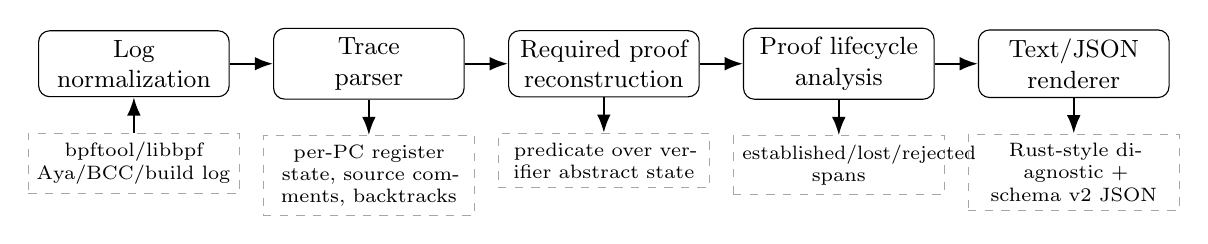
\begin{tikzpicture}[
  stage/.style={rectangle, rounded corners, draw, align=center, minimum height=0.62cm, minimum width=2.42cm, font=\small},
  fact/.style={rectangle, draw=gray!70, dashed, align=center, minimum width=2.45cm, text width=2.45cm, font=\scriptsize},
  arr/.style={-Latex, thick},
  node distance=0.45cm and 0.55cm
]
\node[stage] (log) {Log\\normalization};
\node[stage, right=of log] (parse) {Trace\\parser};
\node[stage, right=of parse] (proof) {Required proof\\reconstruction};
\node[stage, right=of proof] (life) {Proof lifecycle\\analysis};
\node[stage, right=of life] (render) {Text/JSON\\renderer};

\draw[arr] (log) -- (parse);
\draw[arr] (parse) -- (proof);
\draw[arr] (proof) -- (life);
\draw[arr] (life) -- (render);

\node[fact, below=of log] (f1) {bpftool/libbpf\\Aya/BCC/build log};
\node[fact, below=of parse] (f2) {per-PC register state, source comments, backtracks};
\node[fact, below=of proof] (f3) {predicate over verifier abstract state};
\node[fact, below=of life] (f4) {established/lost/rejected spans};
\node[fact, below=of render] (f5) {Rust-style diagnostic + schema v2 JSON};

\draw[arr] (f1) -- (log);
\draw[arr] (parse) -- (f2);
\draw[arr] (proof) -- (f3);
\draw[arr] (life) -- (f4);
\draw[arr] (render) -- (f5);
\end{tikzpicture}
\caption{\sys pipeline。输入是现有工具产生的日志；输出是面向人和工具的诊断。}
\label{fig:pipeline}
\end{figure*}

\subsection{Log normalization}

不同 eBPF 工具有不同日志外壳。bpftool 的 \code{-d} 输出包含 libbpf debug 行；libbpf C loader 可能把 verifier buffer 打到 stderr；Aya 和 BCC 通常把错误包装成语言异常或 logger 输出；CI 日志还会混入 build output。Normalizer 的职责是保留完整上下文，同时尽可能提取 verifier region。它不要求日志必须是纯 verifier 文本；只要其中包含 verifier state 和 terminal error，就可以进入下一阶段。

\subsection{Trace parser}

Trace parser 将日志中的 BPF 指令、寄存器状态和源码注释解析成统一结构。核心字段包括：
\begin{itemize}
  \item instruction pc、opcode、mnemonic；
  \item 每个 live register 的 type、id、offset、range、scalar bounds、\code{tnum}；
  \item verifier terminal error 的 line 和 pc；
  \item BTF/source annotation，如 \code{; if (x > data\_end) @ prog.c:42}；
  \item \code{mark\_precise} 或 verifier backtrack 链。
\end{itemize}

Parser 的失败必须是 non-fatal。即使某些状态 token 是新内核格式，\sys 也应尽量保留 terminal diagnostic，而不是因为解析一个辅助字段失败而不给用户输出。

\subsection{Required proof reconstruction}

Required proof 是在拒绝点必须成立的 verifier 抽象状态谓词。它由两个信息源共同决定：terminal error 给出 proof family，拒绝点寄存器状态给出参数。表~\ref{tab:proof-families} 总结当前设计覆盖的主要 proof family。

\begin{table*}[t]
\centering
\small
\caption{Required proof family。每个 family 都映射到 verifier 抽象状态上的谓词，而不是只映射到错误字符串。}
\label{tab:proof-families}
\begin{tabularx}{\textwidth}{@{}l l X X@{}}
\toprule
Family & 典型错误 & Required proof & 主要帮助方向 \\
\midrule
packet bounds & invalid access to packet & pointer type is pkt 且 range 覆盖 access & 在同一路径上检查 \code{data + size <= data\_end} \\
scalar range & unbounded min/max value & scalar 有非负且有限边界 & mask/clamp/rewrite arithmetic \\
nullable pointer & map\_value\_or\_null deref & nullable pointer 在使用处分支内非空 & null check 后在同分支使用 \\
stack readability & invalid indirect read from stack & 所有读取字节已初始化 & 初始化完整 stack object \\
reference lifecycle & unreleased reference id & 所有路径释放 reference & cleanup path 或 structured goto \\
helper capability & helper not allowed & program type/kernel 支持 helper & 换 program type/kernel/config \\
pointer provenance & invalid mem access scalar & 使用处仍是 verifier pointer type & 保持 pointer provenance 或重新派生 \\
verifier budget & complexity/loop/state limit & 状态空间在 verifier 预算内 & 拆分程序、tail call、简化循环 \\
\bottomrule
\end{tabularx}
\end{table*}

\subsection{Proof lifecycle analysis}

给定 required proof \(P\)，\sys 在 trace 中计算每个 instruction state 对 \(P\) 的状态：unknown、satisfied、violated。状态序列产生生命周期事件：
\[
unknown \rightarrow satisfied \rightarrow violated \rightarrow rejected
\]
其中 \(satisfied \rightarrow violated\) 的第一条转移就是 proof lost witness。若序列中从未出现 satisfied，则诊断为 proof never established。
图~\ref{fig:lifecycle} 展示这种状态机直觉，图~\ref{fig:algorithm} 给出当前实现使用的核心伪代码。

\begin{figure}[t]
\centering
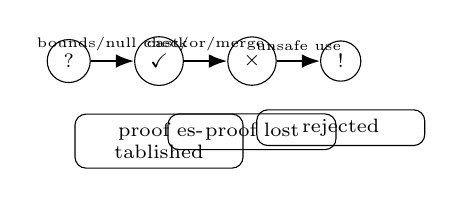
\begin{tikzpicture}[
  dot/.style={circle,draw,minimum size=0.43cm,font=\scriptsize},
  event/.style={rectangle,rounded corners,draw,align=center,font=\scriptsize,text width=1.9cm},
  arr/.style={-Latex,thick},
  node distance=0.55cm
]
\node[dot] (u) {?};
\node[dot, right=of u] (s) {$\checkmark$};
\node[dot, right=of s] (l) {$\times$};
\node[dot, right=of l] (r) {!};
\draw[arr] (u) -- node[above,font=\tiny]{bounds/null check} (s);
\draw[arr] (s) -- node[above,font=\tiny]{cast/or/merge} (l);
\draw[arr] (l) -- node[above,font=\tiny]{unsafe use} (r);
\node[event, below=0.35cm of s] {proof established};
\node[event, below=0.35cm of l] {proof lost};
\node[event, below=0.35cm of r] {rejected};
\end{tikzpicture}
\caption{Proof lifecycle。核心诊断不是最终拒绝点，而是 proof 在轨迹中的生命周期。}
\label{fig:lifecycle}
\end{figure}

Proof lifecycle analysis 需要处理 register lineage。Verifier 寄存器名是物理寄存器；LLVM 会在多条指令间拷贝和复用值。若 required proof 关注的是 \code{R5} 的 pointer provenance，但 \code{R5} 来自 \code{R2} 的 copy，\sys 需要把 proof 追溯到 copy 源头。当前实现覆盖基本 copy、move、ALU 修改和 branch merge 的保守 lineage；未来会进一步利用 object CFG。
这一分析是 best-effort localization，而不是新的 sound verifier。它只解释当前日志中 verifier 已经暴露的抽象状态。若路径合并、alias 或新内核 state token 无法解析，\sys 会退化为 terminal diagnostic，并在 metadata 中记录解析缺口。

\begin{figure}[t]
\begin{lstlisting}[style=tinycode]
diagnose(log):
  trace = parse_verifier_trace(log)
  err   = terminal_error(trace)
  P     = infer_required_proof(err, state_at(err.pc))
  env   = empty_lineage()
  events = []
  status = UNKNOWN

  for insn in trace.instructions:
    env = update_lineage(env, insn)
    st  = project_state(trace.state_at(insn.pc), env, P.regs)
    now = eval(P, st)

    if status == UNKNOWN and now == SAT:
      events += established(insn, P, st)
    if status == SAT and now == VIOLATED:
      events += lost(insn, P, st)
    status = transition(status, now)

  events += rejected(err.pc, err.message)
  return render(events, P, trace.source_spans)
\end{lstlisting}
\caption{Proof lifecycle analysis 的核心伪代码。\code{eval} 把 required proof 投影到当前抽象状态；\code{update\_lineage} 维护寄存器 copy/ALU/merge 的保守别名；\code{transition} 只生成 established/lost 事件，不声称重新证明程序安全。真实实现还包含 fail-soft parsing、case-id handling、object metadata 和 JSON rendering。}
\label{fig:algorithm}
\end{figure}

\subsection{Rendering and integration}

Text renderer 采用 Rust-style multi-span 结构：error id、failure class、primary span、related spans、verifier evidence、required proof 和 help。JSON renderer 输出同一事实的 \code{bpfix.diagnostic/v2} schema，供 CI、编辑器和 agent 消费。设计原则是：text 对人友好，JSON 对工具稳定；二者来自同一个 diagnostic object，避免出现“文档里一种解释，工具里另一种解释”。

\section{实现}
\label{sec:implementation}

\sys 当前实现是 Rust workspace，包括面向用户的 \code{bpfix} CLI 和底层 \code{bpfanalysis} crate。实现遵循三个工程约束。
表~\ref{tab:impl} 总结模块边界，表~\ref{tab:impl-status} 则把 proof family 的实现状态和缺口显式列出，避免把设计目标误写成已经完成的能力。

\textbf{Log-first。} \code{bpfix [LOG]} 是默认入口。没有参数时读 stdin；输入可以是 verifier log、build log、bpftool/libbpf/Aya/BCC 混合 log，或者 evaluation 用的 benchmark YAML。YAML 只抽取 verifier log 和 case id，运行时诊断不读取 benchmark label，避免 oracle 泄漏。

\textbf{Object optional。} \code{--object prog.o} 可以增强 bytecode CFG 和 section metadata，但不是基本诊断的前提。没有 object 时，\sys 仍基于日志输出 proof-oriented diagnosis；有 object 时，系统尝试把 verifier pc 对齐到 object section site，并在 JSON metadata 中记录成功数量或 non-fatal 错误。

\textbf{Fail-soft。} Verifier 日志格式随内核版本变化。实现中，无法解析个别 state token、object parse 失败、source annotation 缺失，都不应阻断 terminal diagnostic。用户最需要的是看到 required proof 和 rejected evidence；增强字段失败以 warning 形式进入 metadata。

\begin{table}[t]
\centering
\small
\caption{实现模块和职责。}
\label{tab:impl}
\begin{tabularx}{\columnwidth}{@{}l X@{}}
\toprule
路径 & 职责 \\
\midrule
\code{crates/bpfix} & CLI、分类、diagnostic object、text/JSON rendering \\
\code{crates/bpfanalysis} & verifier state parser、BPF instruction/CFG analysis \\
\code{bpfix-bench} & replayable corpus、manifest、case harness \\
\code{examples} & bpftool/libbpf/Aya/BCC/CI/editor 集成示例 \\
\code{vendor/libbpf} & local libbpf submodule for benchmark loaders \\
\bottomrule
\end{tabularx}
\end{table}

\begin{table*}[t]
\centering
\small
\caption{当前 proof-family implementation status。Status 区分 classifier、lifecycle 和 localization，避免把 error recognizer 误读成完整 root-cause proof。}
\label{tab:impl-status}
\begin{tabularx}{\textwidth}{@{}l l X X@{}}
\toprule
Proof family & status & 当前信号 & 主要缺口 \\
\midrule
packet bounds & classifier implemented, localization partial & \code{BPFIX-E001}，packet range 和 rejected span & false positive 与 source bug 的区分仍依赖外部证据 \\
nullable pointer & classifier implemented, lifecycle partial & \code{BPFIX-E002}，nullable type 和 deref error & 尚未做完整 CFG dominance proof \\
stack readability & classifier implemented, byte tracking partial & \code{BPFIX-E003}，uninitialized/stack-read terminal error & 字节级初始化轨迹仍是 coarse parsing \\
reference lifecycle & classifier implemented, path cleanup partial & \code{BPFIX-E004}，unreleased reference id & cleanup path localization 还不完整 \\
scalar range & classifier implemented, source/lowering routing partial & \code{BPFIX-E005}，unbounded min/max、map/packet bound evidence & 容易把 source bug 和 lowering artifact 混淆 \\
pointer provenance & classifier implemented, lineage partial & \code{BPFIX-E006}，invalid scalar pointer 和 basic lineage span & pointer-preserving lowering witness 覆盖不足 \\
helper/environment & classifier implemented & \code{BPFIX-E009}，helper、program type、BTF/kfunc/JIT routing & 细分到具体 kernel feature 的解释仍需扩展 \\
dynptr/kfunc/iterator & classifier partial & \code{BPFIX-E012} 覆盖一部分 dynptr selftest & lifecycle span 和错误子类仍需扩展 \\
verifier budget & classifier implemented & \code{BPFIX-E018}，program-too-large、combined stack、complexity limit & 如何指向状态爆炸根源仍是 partial localization \\
\bottomrule
\end{tabularx}
\end{table*}

\subsection{CLI and output schema}

CLI help 当前暴露的主模型是：
\begin{lstlisting}[style=tinycode]
Usage: bpfix [OPTIONS] [INPUT]

Arguments:
  [INPUT] verifier/build/bpftool/libbpf/Aya/BCC log

Options:
  --object <OBJECT>
  --format <text|json|both>  [default: text]
\end{lstlisting}

JSON schema v2 包含 \code{error\_id}、\code{failure\_class}、\code{required\_proof}、\code{source\_span}、\code{related\_spans}、\code{evidence}、\code{help} 和 metadata。我们刻意使用 \code{help} 而不是 \code{candidate\_repairs}，因为当前系统解释 verifier 需要的证明和可能的代码方向，但不承诺自动 patch。

\subsection{Benchmark replay and local libbpf}

Benchmark 中的 kernel selftest cases 需要 userspace loader。此前 replay 环境的 85 个失败不是“没有真实 eBPF 程序”，而是 loader 链接 host \code{-lbpf} 失败。我们将 selftest loader 改为通过 \code{bpfix-bench/libbpf.mk} 构建并链接本地 \code{vendor/libbpf} static library。这样 benchmark replay 不依赖系统安装 \code{libbpf-dev}，减少环境噪声。修复后完整 validator 在当前主机上通过 235/235 cases。

\section{Evaluation}
\label{sec:evaluation}

本文当前版本评估两个层次：artifact validity 和 diagnostic capability。Artifact validity 问题是 \code{bpfix-bench} 是否真的能在本地重放 verifier reject；diagnostic capability 问题是当前 Rust \code{bpfix} 是否能稳定读取 replay log、输出结构化 JSON、产生 required proof/help，并在多大范围内识别具体 error id 和 proof lifecycle。
表~\ref{tab:eval-claims} 是评测段的 claim ledger：只有 replay validity 和 log-first robustness 被当前证据完全支撑，其余诊断正确性 claim 都按 partial/open 处理。

\begin{table*}[t]
\centering
\small
\caption{Evaluation claim ledger。表中把当前已验证证据和最终 OSDI claim 分开，避免把 pilot coverage 写成完整正确性结论。}
\label{tab:eval-claims}
\begin{tabularx}{\textwidth}{@{}l X X l@{}}
\toprule
Claim & 需要证明什么 & 当前证据 & 状态 \\
\midrule
C1 replayable corpus & benchmark case 能在固定环境中重新触发 verifier reject & validator 235/235 pass，selftest loader 85/85 local libbpf link & supported \\
C2 log-first robustness & 用户给现有工具日志时，\sys 能 fail-soft 输出诊断对象 & 235/235 replay log 产生 parseable JSON、primary span、evidence 和 help & supported \\
C3 proof-family coverage & 常见 verifier failure 能映射到具体 error id 和 required proof & 235/235 known error id，99/235 有 related proof spans & partial \\
C4 taxonomy routing & 系统能区分 source bug、lowering artifact、verifier false positive 和环境/配置失败 & coarse failure-class 与 taxonomy agreement 为 217/235；lowering artifact recall 为 12/24，verifier false positive recall 为 6/9，environment recall 为 10/11，limit recall 为 4/4 & partial \\
C5 user advantage & 与 terminal-message baseline 相比，用户得到更多结构化定位信息 & label-proxy baseline 显示 root-pc exact 101/140；60-case blind audit 中 \sys root exact/near 为 18/26 和 21/27，correct help 为 24/60 和 23/60 & partial \\
\bottomrule
\end{tabularx}
\end{table*}

\begin{enumerate}
  \item \textbf{Replay reliability：} benchmark case 是否能在固定环境中重建 verifier reject？
  \item \textbf{Parser/renderer robustness：} \sys 是否能对每条 fresh replay log 输出 parseable JSON？
  \item \textbf{Diagnostic coverage：} 当前 error catalog 覆盖多少 case，哪些 case 仍落到 unsupported 或 fallback family？
  \item \textbf{Proof-span coverage：} \sys 是否能输出 rejected span、evidence、help 和 related proof spans？
  \item \textbf{Baseline proxy：} 与只看 terminal error 的 dictionary baseline 相比，\sys 是否提供额外结构化定位信息？
  \item \textbf{Tool usability：} 用户是否能通过现有 bpftool/libbpf/Aya/BCC/CI 工作流接入？
\end{enumerate}

\begin{table}[t]
\centering
\small
\caption{Artifact validity：当前仓库中已验证的运行状态。}
\label{tab:current-validation}
\begin{tabularx}{\columnwidth}{@{}l l X@{}}
\toprule
检查 & 结果 & 说明 \\
\midrule
Benchmark replay & 235/235 pass & validator 重新构建、加载并捕获 reject \\
Rust unit/CLI tests & 59/59 pass & parser、diagnostic、CLI 行为 \\
Selftest loader build & 85/85 pass & local libbpf static link \\
Examples syntax & pass & shell、JSON、Python、Rust snippet check \\
\bottomrule
\end{tabularx}
\end{table}

\begin{table}[t]
\centering
\small
\caption{Replay environment used for the 235/235 validation。Benchmark 仍是环境敏感的，表中版本定义本文所有 replay 和 diagnostic 数字的运行上下文。}
\label{tab:replay-env}
\begin{tabularx}{\columnwidth}{@{}l X@{}}
\toprule
组件 & 版本或配置 \\
\midrule
kernel & \code{6.15.11-061511-generic} \\
clang/LLVM & Ubuntu clang \code{18.1.3}，target \code{x86\_64-pc-linux-gnu} \\
bpftool & \code{v7.7.0}，using libbpf \code{v1.7} \\
benchmark env id & \code{kernel-6.15.11-clang-18-log2} \\
local libbpf & \code{vendor/libbpf} \code{dd92bef} (\code{v1.7.0-16-gdd92bef}) \\
\bottomrule
\end{tabularx}
\end{table}

\begin{table}[t]
\centering
\small
\caption{当前 Rust \code{bpfix --format json} 在 235 条 replay log 上的覆盖。}
\label{tab:rust-coverage}
\begin{tabularx}{\columnwidth}{@{}l r X@{}}
\toprule
指标 & cases & 说明 \\
\midrule
JSON 成功 & 235 & 所有 replay log 都产生 parseable diagnostic JSON \\
primary span & 235 & 每条输出 rejected/source 或 bytecode span \\
evidence & 235 & 每条输出 verifier evidence \\
help & 235 & 每条输出至少一条 proof-oriented help \\
known error id & 156 & 非 \code{BPFIX-UNKNOWN}，覆盖仍需扩展 \\
related proof spans & 91 & 有 proof established/lost 或相关 lifecycle span \\
\bottomrule
\end{tabularx}
\end{table}

\begin{table}[t]
\centering
\small
\caption{当前 Rust diagnostic 的 failure-class 输出分布。该分布是系统输出，不等同于 ground-truth taxonomy。}
\label{tab:runtime-classes}
\begin{tabular}{lr}
\toprule
输出 failure class & cases \\
\midrule
\code{source\_bug} & 167 \\
\code{lowering\_artifact} & 48 \\
\code{environment\_or\_configuration} & 16 \\
\code{verifier\_limit} & 4 \\
\bottomrule
\end{tabular}
\end{table}

\begin{table}[t]
\centering
\small
\caption{Ground-truth taxonomy 与当前 runtime failure-class 的 confusion。列是 \sys 输出，行是 \code{case.yaml} taxonomy。}
\label{tab:taxonomy-confusion}
\begin{tabular}{lrrrr}
\toprule
Ground truth & source & lowering & env & limit \\
\midrule
source bug & 140 & 42 & 5 & 0 \\
lowering artifact & 20 & 4 & 0 & 0 \\
environment/config & 0 & 0 & 11 & 0 \\
false positive & 7 & 2 & 0 & 0 \\
verifier limit & 0 & 0 & 0 & 4 \\
\midrule
total output & 167 & 48 & 16 & 4 \\
\bottomrule
\end{tabular}
\end{table}

\begin{table*}[t]
\centering
\small
\caption{Per-source diagnostic coverage。Agreement 是 coarse failure-class 与 benchmark taxonomy 相同的 case 数；它不是完整 root-cause correctness。}
\label{tab:per-source-coverage}
\begin{tabularx}{\textwidth}{@{}l r r r r X@{}}
\toprule
source & cases & agreement & known id & related spans & interpretation \\
\midrule
GitHub commit & 46 & 20 & 26 & 18 & 真实项目回归和 compiler/lowering 相关 case 多，routing 最难 \\
GitHub issue & 18 & 10 & 15 & 13 & 日志较短但用户上下文明确，span coverage 较高 \\
kernel selftest & 85 & 74 & 53 & 17 & terminal error 稳定，现代 dynptr/kfunc/iterator span 仍不足 \\
Stack Overflow & 86 & 55 & 62 & 43 & 用户问题覆盖 packet、map、helper 和 verifier corner case \\
\midrule
total & 235 & 159 & 156 & 91 & agreement 67.7\%，known-id 66.4\%，related-span 38.7\% \\
\bottomrule
\end{tabularx}
\end{table*}

\subsection{Artifact validity}

Replay validator 的通过证明了两件事。第一，corpus 中的 235 个 case 不是静态文本集合，而是能在当前环境中重新构建、重新加载、重新产生 verifier reject 的程序集合。第二，kernel selftest 子集不再被 host \code{-lbpf} 依赖阻塞；85 个 selftest loader 都通过本地 \code{vendor/libbpf} 构建并链接。这一点对 evaluation 很关键：如果 replay 环境不稳定，后续诊断准确率没有可信分母。
表~\ref{tab:current-validation} 汇总了这个 artifact validity gate。表~\ref{tab:replay-env} 固化本次运行环境，避免把 kernel/compiler 相关结果误解成跨版本不变结论。

\subsection{Current diagnostic capability}

表~\ref{tab:rust-coverage} 是当前 Rust CLI 的真实覆盖状态。所有 235 条 replay log 都能被 \code{bpfix --format json} 处理，说明 log normalization、terminal error handling、JSON rendering 和 fail-soft 策略已经达到工具可用的最低门槛。所有输出都包含 primary span、evidence 和 help，符合“用户至少能得到下一步检查方向”的 UX 目标。
表~\ref{tab:runtime-classes} 给出 runtime failure-class 的输出分布，它是系统输出而不是 ground truth。

同时，覆盖仍不完整。当前 replay logs 已全部避开 \code{BPFIX-UNKNOWN}/fallback family，并在 235/235 case 上给出具体 error id；但 related proof spans 只有 99/235，说明 proof lifecycle reconstruction 已在一部分 case 上工作，还不是所有 case 的默认能力。因此，当前论文不应声称“完整自动 root-cause localization”；更可信的 claim 是：\sys 建立了 log-first diagnostic architecture，并已在 235 个 replayable reject 上证明鲁棒性，在 235 个 case 上给出具体 error id，在 99 个 case 上给出 proof lifecycle span。

表~\ref{tab:taxonomy-confusion} 进一步给出 coarse routing 的真实状态。当前 runtime failure-class 与 benchmark taxonomy 在 217/235 个 case 上相同。这个数字不能被写成最终诊断准确率，因为 taxonomy 只有粗粒度类别，而最终诊断还必须评价 required proof、causal mechanism、root span 和 false claim。它的价值在于暴露实现缺口：environment/configuration、verifier limit、一半 lowering artifact 和 6/9 verifier false positive 已能被当前 classifier 路由，但仍有 3 个 false positive 被当作 source/lowering 类处理，scalar range 与 pointer provenance case 也仍会把部分 source bug 和 lowering artifact 混在一起。表~\ref{tab:per-source-coverage} 显示这种缺口在真实项目和 Stack Overflow case 上更明显，而 kernel selftest 的 terminal message 更规范，coarse agreement 更高。

\subsection{Baselines}

我们把 baseline 分成已运行的 label-proxy baseline 和正式 submission 前必须补的 human-scored baseline。已运行 baseline 是 terminal dictionary：只看 \code{case.yaml} 中的 terminal error，用一组 regex 输出 error id、failure class 和粗略 next action。它代表 final-message translator 的下界，不读取 full verifier trace、source annotation 或 object metadata。表~\ref{tab:proxy-baseline} 给出结果：\sys 当前在 known error id、coarse taxonomy agreement、macro-F1、lowering recall、verifier false-positive recall、primary span、related proof spans 和 root-pc localization 上超过 terminal dictionary；terminal dictionary 在 next-action proxy 上仍略高，说明 action proxy 噪声较大，help quality 仍必须用 human scoring 支撑。这个结果支持“\sys 提供 terminal-only baseline 没有的结构化定位上下文和部分 coarse routing 增量”，但仍不等价于完整自动 root-cause correctness。

完整 baseline 计划仍包括 raw verifier log、Pretty Verifier 类工具和 LLM+raw-log，并用同一个 oracle 比较 required proof、root-cause span、help quality、triage time 和输出稳定性。为减少纯 proxy 指标的偏差，我们进一步构造 60-case 分层样本，并让两个独立 scorer 在匿名方法 \code{M1/M2/M3} 上做 blind audit。样本包含全部 minority classes：24 个 lowering artifact、11 个 environment/configuration、9 个 false positive、4 个 verifier limit，以及 12 个 source bug；结果记录在 \code{docs/evaluation/blind-audit-results.md}。表~\ref{tab:blind-audit} 显示 \sys 在 root localization 和 help quality 上明显优于 raw terminal 和 terminal dictionary，但 unsafe help 仍有 14/60，说明当前结果支持 partial user-advantage claim，而不是完整诊断正确性。

\begin{table*}[t]
\centering
\small
\caption{Label-proxy baseline results on 235 replay logs。命令为 \code{python3 docs/evaluation/evaluate\_diagnostics.py --confusion}。Terminal dictionary 只使用 \code{case.yaml} 中的 terminal error，不读取 full verifier trace 或 source spans。}
\label{tab:proxy-baseline}
\begin{tabularx}{\textwidth}{@{}l r r X@{}}
\toprule
Metric & \sys full log & terminal dictionary & interpretation \\
\midrule
known error id & 235/235 & 145/235 & \sys 避免 fallback/unknown，并覆盖 dynptr、environment、limit、lowering 和 verifier-precision families \\
error-id exact & 60/235 & 43/235 & label error id 比 runtime catalog 更细，二者都偏低 \\
taxonomy agreement & 217/235 & 199/235 & \sys 利用 full-log proof/lowering/precision signals 提升 coarse routing，但不是完整 root-cause accuracy \\
taxonomy macro-F1 & 0.858 & 0.558 & minority-class routing 明显改善，但仍不是完整 help correctness \\
lowering recall & 12/24 & 0/24 & terminal-only 无法识别 verifier-visible lowering artifacts \\
environment recall & 10/11 & 11/11 & 显式 capability pattern 覆盖多数 env cases，但仍有边界 case 需要 object/environment context \\
verifier false-positive recall & 6/9 & 0/9 & terminal-only 无法区分 verifier precision limit 与普通 source bug \\
verifier-limit recall & 4/4 & 4/4 & 显式 budget pattern 已覆盖当前 limit cases \\
primary span emitted & 235/235 & 0/235 & terminal-only baseline 不产生结构化 span \\
related proof spans & 99/235 & 0/235 & \sys 的主要增量是 proof lifecycle context \\
root pc exact, labeled n=140 & 101/140 & 0/140 & span pc 候选命中 label root instruction \\
root pc within 5, labeled n=140 & 120/140 & 0/140 & coarse localization 已可度量，但不是完整 source-span correctness \\
next-action proxy exact & 116/235 & 124/235 & 自动 action proxy 噪声较大，需 expert/user study 确认 help quality \\
\bottomrule
\end{tabularx}
\end{table*}

\begin{table*}[t]
\centering
\small
\caption{Independent blind audit on a 60-case stratified sample。Scorer A/B 分别独立评分；\code{M1} 是 raw terminal message，\code{M2} 是 terminal dictionary，\code{M3} 是 \sys full-log diagnostic。}
\label{tab:blind-audit}
\begin{tabularx}{\textwidth}{@{}l l r r r X@{}}
\toprule
Metric & Method & exact/correct & partial/near & miss/unsafe/none & interpretation \\
\midrule
required proof & M1 & 0/0 & 60/60 & 0/0 & terminal symptom 只给 partial proof context \\
required proof & M2 & 8/15 & 43/28 & 9/17 & dictionary 可识别部分 obvious proof family \\
required proof & M3 & 16/22 & 42/20 & 2/18 & \sys 更常给出具体 required proof，但 scorer 对 UNKNOWN/partial 边界分歧较大 \\
\midrule
root localization & M1 & 0/0 & 0/0 & 26/27 miss, 34/33 na & raw terminal 没有 root span \\
root localization & M2 & 0/0 & 0/0 & 26/27 miss, 34/33 na & dictionary baseline 也没有 root span \\
root localization & M3 & 15/16 & 3/5 & 8/6 miss, 34/33 na & \sys 在有 root oracle 的 case 中定位优势最明显 \\
\midrule
help quality & M1 & 0/0 & 0/0 & 60/60 none & raw terminal 不给 help \\
help quality & M2 & 0/0 & 46/50 & 14/10 unsafe & generic action 有方向但不可定位 \\
help quality & M3 & 24/23 & 22/23 & 14/14 unsafe & \sys 给出最多 correct help，但 unsafe case 仍需扩展 catalog \\
\bottomrule
\end{tabularx}
\end{table*}

\subsection{Remaining OSDI evaluation gap}

要达到完整 OSDI submission，仍需要补两类实验。第一，将 60-case blind audit 扩展到更大分层样本，并加入真实 eBPF 开发者或 reviewer，而不是只依赖项目内独立 scorer。第二，在同一批 fresh replay log 上运行 raw-log、Pretty Verifier 或等价工具、LLM+raw-log，并比较 required proof、localization、help quality 和 triage time。当前草稿已经给出可复现 label-proxy baseline、60-case blind audit 和初步系统数据，足以支持“结构化定位和 help 上有增量”的 limited claim；完整 headline user advantage 仍需要这些外部人工 oracle 才能作为最终论文 claim。这个范围收紧反而是 submission 必需的：如果只报告 235/235 JSON success，会像 artifact report；只有把 proof correctness、localization 和用户任务指标放到同一评测矩阵里，\sys 的系统贡献才可被 reviewer falsify。

\subsection{用户任务指标}

对于开源工具，最终指标应接近用户任务：给定一个 verifier reject，用户是否能在 30 秒内知道该跑什么命令；看到输出后，是否知道下一步检查哪一行、需要建立什么 proof、问题是否可能是环境而非源码。60-case blind audit 已经说明 \sys 在 root localization 和 correct help 上优于 terminal-only baseline；下一步需要让 eBPF 开发者在 20--30 个真实案例上比较 raw log、baseline 和 \sys 的 triage 时间与修改方向质量。

\section{开源工具体验}

\sys 不应只是 paper artifact。为此我们把用户体验当作系统设计的一部分，而不是 README 的附属物。

\textbf{默认命令最小化。} 主路径是 \code{bpfix [LOG]}，默认 plain text。用户不用先选择 mode、benchmark 或 label。

\textbf{集成示例覆盖真实工具。} \code{examples/} 按工具分目录：\code{bpftool/}、\code{make/}、\code{libbpf-c/}、\code{libbpf-rs/}、\code{aya/}、\code{bcc/}、\code{ci/}、\code{editor/}。示例展示如何捕获 verifier log，而不是发明新的加载方式。

\textbf{JSON 面向 downstream tools。} CI 和 editor 示例使用 \code{--format json}，而本地调试文档默认 plain text。这避免普通用户被 schema 干扰，也让工具集成有稳定接口。

\textbf{Benchmark 退到开发者路径。} \code{bpfix-bench} 是回归和评价基础，但 README 前半部分不要求用户理解它。用户先学会诊断自己的 log，维护者再用 benchmark 保证诊断质量。

\FloatBarrier

\section{相关工作}

\textbf{eBPF verifier 和开发难度。} Gershuni 等人形式化了 eBPF verifier 的静态分析性质~\cite{gershuni2019simple}。HotOS 和开发者研究指出 kernel extension verification 的可用性问题和 eBPF 开发挑战~\cite{hotos2023verif,deokar2024}。这些工作说明 verifier 是安全基础，也是开发者瓶颈。\sys 关注其中最直接的 UX 层：当 verifier 已经拒绝程序时，如何把 proof trace 转换成可行动诊断。

\textbf{语言和 verifier gap。} Rex 通过新的语言/运行时设计缩小 language-verifier gap~\cite{rex2025}。K2 和 SimpleBPF 等工作从优化或生成角度处理 eBPF 程序~\cite{k22023,simplebpf2025}。与这些系统不同，\sys 不要求用户换语言或生成程序，而是服务现有 C/Rust/Aya/libbpf/BCC 代码。

\textbf{Verifier 错误解释。} Pretty Verifier 和 verifier error dictionary 类项目改善了错误文本可读性~\cite{prettyverifier2025,ebpfverifdict}。它们通常以最终错误消息为中心。\sys 的区别是从完整 trace 中重建 proof lifecycle，并输出 proof established/lost/rejected 的多 span 解释。

\textbf{Compiler diagnostics。} Rust 编译器诊断的价值在于使用类型检查、borrow checking 和 span 信息输出结构化 error、note 和 help~\cite{rustdiag2016,errormessages2014}。\sys 借鉴这种输出形态，但事实来源不是编译器 IR，而是 verifier 抽象状态轨迹和可选 BPF object CFG。

\section{局限性与讨论}

\textbf{Log 质量限制。} 如果 loader 没有开启 verifier log，或日志只保留最终 errno，\sys 无法重建 proof lifecycle。示例和文档必须优先教用户如何捕获完整 log。

\textbf{跨内核差异。} Verifier 行为随内核版本变化。同一源码在不同 kernel、BTF、helper 支持下可能接受或拒绝。\sys 诊断当前日志，不声称跨内核 root cause 一定一致。

\textbf{False positive 判断需要外部证据。} \sys 可以识别“看起来像 verifier 保守性”的模式，但严格判定 verifier false positive 通常需要上游 patch、maintainer 讨论或等价语义证明。当前系统应谨慎输出“likely false positive”，并保留 evidence。

\textbf{不是自动修复。} \sys 输出 help 和 proof requirement，不自动改源码。自动 patch 需要语义保持、编译验证和 verifier replay，是独立系统问题；把它混入当前 CLI 会损害用户信任。

\section{结论}

eBPF verifier 失败不是普通错误字符串，而是安全证明失败。本文提出 \sys，将 verbose verifier log 视为 proof trace，重建 required proof 和 proof lifecycle，并把 opaque log 转换成 Rust-style multi-span 诊断。通过 235 个 replayable case 的 characterization，我们展示真实失败覆盖 source bug、lowering artifact、environment/configuration、verifier false positive 和 verifier limit。通过 label-proxy baseline 和 60-case blind audit，我们展示当前 \sys 的主要增量是结构化 root localization 和 proof-oriented help，同时也暴露了 false-positive、alignment 和 verifier-specific lifecycle case 上的 unsafe help。通过 log-first CLI、stable JSON 和跨工具 examples，\sys 目标是成为可用的开源诊断工具，而不是只服务论文评估的研究原型。

\bibliographystyle{plain}
\bibliography{references}

\end{document}
